% Présentation des éditions jusque là et des différentes hypothèses sur la transmission du texte.
\documentclass[11pt]{beamer}
\graphicspath{{img/}{./}}
\usepackage[french]{babel}
\usepackage{graphicx}
\usepackage{ulem} %Pour biffer du texte \sout{texte barré}
\usepackage{xcolor} 
\usepackage{tabularx}
\usepackage{parallel}
%\usepackage[babelshorthands]{polyglossia}
\usepackage{ragged2e} 


%Allignemebnt droite/gauche
\usepackage{polyglossia}
%\usepackage[babelshorthands]{polyglossia} %[babelshorthands] permet d'avoir les guillemets allemands avec le code "`toto"' et les guillemets français avec le code "<tata">


\usepackage{multirow} 
\setmainlanguage{english}
\usepackage[autostyle]{csquotes}
\MakeOuterQuote{"}
\DeclareQuoteStyle{english}%
    {\textquotedblleft}
    [\textquotedblleft]
    {\textquotedblright}
        [0.05em]
    {\textquoteleft}
    [\textquoteleft]
    {\textquoteright}
% \DeclareQuoteStyle[quotes]{french}
%   {\mkfrenchopenquote{«}}
%   {\mkfrenchclosequote{\nobreakspace»}}
%   {\textquotedblleft}
%   {\textquotedblright}
% \DeclareQuoteStyle[quotes*]{french}
%   {\mkfrenchopenquote{«}}
%   {\mkfrenchclosequote{\nobreakspace»}}
%   {\mkfrenchopenquote{\textquotedblleft}}
%   {\mkfrenchclosequote{\textquotedblright}}
% \DeclareQuoteStyle[guillemets]{french}
%   [\initfrenchquotes]
%   {\mkfrenchopenquote{«}}
%   [\mkfrenchopenquote{«}]
%   {\mkfrenchclosequote{\nobreakspace»}}
%   {\mkfrenchopenquote{«}}
%   [\mkfrenchopenquote{«}]
%   {\mkfrenchclosequote{\nobreakspace»}}
% \DeclareQuoteStyle[guillemets*]{french}
%   [\initfrenchquotes]
%   {\mkfrenchopenquote{«}}
%   [\mkfrenchopenquote{\nobreakspace»}]
%   {\mkfrenchclosequote{\nobreakspace»}}
%   {\mkfrenchopenquote{«}}
%   [\mkfrenchopenquote{\nobreakspace»}]
%   {\mkfrenchclosequote{\nobreakspace»}}




\setotherlanguage{greek}
\newfontfamily\greekfont[Script=Greek]{Linux Libertine O}
\newfontfamily\greekfontsf[Script=Greek]{Linux Libertine O}
\setotherlanguage{hebrew}
\newfontfamily{\hebrewfont}[Script=Hebrew, Path=./fonts/]{SBL_Hbrw.ttf}
\newfontfamily{\hebrewfontsf}[Script=Hebrew]{Miriam CLM}
\newfontfamily{\hebrewfonttt}[Script=Hebrew]{Miriam Mono CLM}
\setotherlanguage{syriac}
\newfontfamily\syriacfont[Script=Syriac, Path=./fonts/]{EstrangeloEdessa.ttf}

\usepackage{booktabs} % Allows the use of \toprule, \midrule and \bottomrule for better rules in tables
%% Allow the use of tcolorbox
\usepackage[skins]{tcolorbox}
%\usetheme{default}
%\usetheme{AnnArbor}
%\usetheme{Antibes}
%\usetheme{Bergen}
%\usetheme{Berkeley}
%\usetheme{Berlin}
%\usetheme{Boadilla}
%\usetheme{CambridgeUS}
%\usetheme{Copenhagen}
%\usetheme{Darmstadt}
%\usetheme{Dresden}
%\usetheme{Frankfurt}
%\usetheme{Goettingen}
%\usetheme{Hannover}
%\usetheme{Ilmenau}
\usetheme{JuanLesPins}
%\usetheme{Luebeck}
%\usetheme{Madrid}
%\usetheme{Malmoe}
%\usetheme{Marburg}
%\usetheme{Montpellier}
%\usetheme{PaloAlto}
%\usetheme{Pittsburgh}
%\usetheme{Rochester}
%\usetheme{Singapore}
%\usetheme{Szeged}
%\usetheme{Warsaw}

%----------------------------------------------------------------------------------------
%	SELECT COLOR THEME
%----------------------------------------------------------------------------------------

% Beamer comes with a number of color themes that can be applied to any layout theme to change its colors. Uncomment each of these in turn to see how they change the colors of your selected layout theme.

%\usecolortheme{albatross}
%\usecolortheme{beaver}
%\usecolortheme{beetle}
%\usecolortheme{crane}
%\usecolortheme{dolphin}
%\usecolortheme{dove}
%\usecolortheme{fly}
%\usecolortheme{lily}
%\usecolortheme{monarca}
%\usecolortheme{seagull}
%\usecolortheme{seahorse}
%\usecolortheme{spruce}
%\usecolortheme{whale}
%\usecolortheme{wolverine}

%----------------------------------------------------------------------------------------
%	SELECT FONT THEME & FONTS
%----------------------------------------------------------------------------------------
\setmainfont{cochineal}
% Beamer comes with several font themes to easily change the fonts used in various parts of the presentation. Review the comments beside each one to decide if you would like to use it. Note that additional options can be specified for several of these font themes, consult the beamer documentation for more information.

%\usefonttheme{default} % Typeset using the default sans serif font
\usefonttheme{serif} % Typeset using the default serif font (make sure a sans font isn't being set as the default font if you use this option!)
%\usefonttheme{structurebold} % Typeset important structure text (titles, headlines, footlines, sidebar, etc) in bold
%\usefonttheme{structureitalicserif} % Typeset important structure text (titles, headlines, footlines, sidebar, etc) in italic serif
%\usefonttheme{structuresmallcapsserif} % Typeset important structure text (titles, headlines, footlines, sidebar, etc) in small caps serif

%------------------------------------------------

%\usepackage{mathptmx} % Use the Times font for serif text
%\usepackage{palatino} % Use the Palatino font for serif text


%\usepackage{helvet} % Use the Helvetica font for sans serif text
%\usepackage[default]{opensans} % Use the Open Sans font for sans serif text
%\usepackage[default]{FiraSans} % Use the Fira Sans font for sans serif text
%\usepackage[default]{lato} % Use the Lato font for sans serif text

%----------------------------------------------------------------------------------------
%	SELECT INNER THEME
%----------------------------------------------------------------------------------------

% Inner themes change the styling of internal slide elements, for example: bullet points, blocks, bibliography entries, title pages, theorems, etc. Uncomment each theme in turn to see what changes it makes to your presentation.

%\useinnertheme{default}
%\useinnertheme{circles}
\useinnertheme{rectangles}
%\useinnertheme{rounded}
%\useinnertheme{inmargin}

%----------------------------------------------------------------------------------------
%	SELECT OUTER THEME
%----------------------------------------------------------------------------------------

% Outer themes change the overall layout of slides, such as: header and footer lines, sidebars and slide titles. Uncomment each theme in turn to see what changes it makes to your presentation.

%\useoutertheme{default}
%\useoutertheme{infolines}
%\useoutertheme{miniframes}
%\useoutertheme{smoothbars}
%\useoutertheme{sidebar}
%\useoutertheme{split}
%\useoutertheme{shadow}
%\useoutertheme{tree}
%\useoutertheme{smoothtree}

%\setbeamertemplate{footline} % Uncomment this line to remove the footer line in all slides
%\setbeamertemplate{footline}[page number] % Uncomment this line to replace the footer line in all slides with a simple slide count

%\setbeamertemplate{navigation symbols}{} % Uncomment this line to remove the navigation symbols from the bottom of all slides
\usepackage[style=sbl]{biblatex}


\DeclareSourcemap{
  \maps[datatype=bibtex]{
    \map{
      \step[fieldset=doi, null]
      \step[fieldset=language, null]
      \step[fieldset=issn, null]{}
      \step[fieldset=url, null]{}
      \step[fieldset=isbn, null]{}
      \step[fieldset=eprint, null]{}
    }
  }
}

\addbibresource{references.bib}
%\defbibheading{bibempty}{}

%----------
% Define sectioning
\AtBeginSection[]{
  \begin{frame}
  \vfill
  \centering
  \begin{beamercolorbox}[sep=8pt,center,shadow=true,rounded=true]{title}
    \usebeamerfont{title}\insertsectionhead\par%
  \end{beamercolorbox}
  \vfill
  \end{frame}
}

%-----------

%----------------------------------------------------------------------------------------
%	PRESENTATION INFORMATION
%----------------------------------------------------------------------------------------


\title{Introduction à la critique textuelle}
\author[Frédérique Michèle Rey, Sophie Robert-Hayek]{Frédérique Michèle Rey \& Sophie Robert-Hayek}


\institute[UL]{Université de Lorraine } %\smallskip \textit{frederique.rey@univ-lorraine.fr / sophie.robert@univ-lorraine.fr}}

\date{}
\setbeamertemplate{footline}[frame number]

\usepackage[table]{xcolor}
\usepackage[dvipsnames]{xcolor}
\usepackage{forest}
\usepackage{tikz-qtree}
\usepackage{amsmath}
\usepackage{amsfonts}
\usepackage[font=scriptsize]{caption}
\begin{document}
\title{Les éditions critiques}
\subtitle{Critique textuelle du Nouveau Testament}

\begin{frame}{}
    \titlepage
\end{frame}

\begin{frame}{Plan du cours}
\tableofcontents
\end{frame}



\section{Principes de la critique textuelle}

\begin{frame}{Principes de la critique textuelle}
    \begin{alertblock}{}
        
    \end{alertblock}
\end{frame}

% Comment établir une lecture: workflow
\begin{frame}{Méthode de travail}
    \begin{alertblock}{}
        La \textbf{critique interne} l'étude du variant, afin de l'expliquer :
        \begin{itemize}
        \item S'agit-il d'une variante accidentelle ou délibérée ? 
        \item Comment expliquer les raisons pour le scribe d'avoir produit une telle variante ?
        \item Quels sont les arguments logiques et contextuels pour une leçon plutôt qu'une autre ? 
        \end{itemize}
        % concernent les probabilités de ce qu'un scribe aurait pu faire, intentionnellement ou non, et qui aurait produit une lecture différente
    \end{alertblock}

    \begin{alertblock}{}
        La \textbf{critique externe} consiste en :
        \begin{itemize}
            \item l'étude du reste du manuscrit (stylistique, qualité du texte, datation du manuscrit);
            \item l'étude du nombre de manuscrits et de la qualité des manuscrits présentant la même lecture.
        \end{itemize}
    \end{alertblock}
\end{frame}

\begin{frame}{Méthode de travail}
L'exercice de la critique textuelle se déroule de la façon suivante :
    \begin{enumerate}
        \item Collection des manuscrits;
        \item Réalisation de la collation;
        \item Collection des lectures;
        \item Critique interne des leçons;
        \item Critique externe des manuscrits;
        \item Choix final de la leçon.
    \end{enumerate}
\end{frame}

% Diapositive : Passages Parallèles


\begin{frame}{Choisir une leçon : critique interne}
    Principe fondamentale pour la \textbf{critique interne} (Greenlee, 1964):\\
        \begin{alertblock}{}
        Ces principes peuvent sembler \textbf{contradictoires}, mais il s'agit d'un art \dots
        \textit{A constantly maintained familiarity with New Testament manuscripts themselves is the best training for textual criticism. In textual criticism the pure theoretician has often done more harm than good.} (Alands, les 12 règles de la critique textuelle).
    \end{alertblock}
    
\begin{block}{}
    \textbf{Lecture  probable :} \\
    
    La lecture dont les autres \textbf{dérivent} \textbf{probablement} est considérée comme \textbf{correcte}.
\end{block}
\end{frame}

\begin{frame}{Choisir une leçon : critique interne}

\begin{enumerate}
\item La lecture dont les autres \textbf{dérivent} \textbf{probablement} est considérée comme \textbf{correcte}.

    \item \textbf{Lecture difficile (\textit{lectio difficilior potior}):} une leçon plus difficile est plus probable, car les scribes modifient pour clarifier.
    
    \item \textbf{Lecture courte (\textit{lectio brevior potior}) :} 
    En cas de changement intentionnel, la leçon plus courte est préférable, car un scribe ajoute plutôt qu'il enlève.

    \item \textbf{Lecture longue :} si une omission accidentelle est suspectée, la \textbf{leçon la plus courte est préférable}.
\end{enumerate}

\end{frame}

\begin{frame}{Choisir une leçon : critique interne}

\begin{enumerate}
    \item \textbf{Leçon et passages parallèles :} Dans les variantes où il existe un passage parallèle, la leçon la moins similaire est la plus probable.
    \item \textbf{Leçon et style du texte :} la leçon la plus éloignée du style de l'auteur est moins probable.
\end{enumerate}

\end{frame}


\begin{frame}{Choisir une leçon : critique externe}
    Principes généraux pour la \textbf{critique externe}:
    \begin{itemize}
        \item \textbf{Lister les manuscrits} qui présentent la même leçon;
        \item \textbf{Estimer leur datation}, leur \textbf{type de texte} et leur \og \textbf{qualité} \fg.
    \end{itemize}

    \begin{alertblock}{}
       Le choix de la leçon doit peser à la fois la critique interne et la critique externe afin de prendre une décision.
    \end{alertblock}
\end{frame}

\begin{frame}{Exemple : Luc 24,53}
    \begin{exampleblock}{}
   \textit{Luc 24,53} : ils étaient continuellement dans le temple, louant et bénissant Dieu.\\
   
   L1: \textgreek{αἰνοῦντες}\\
   L2: \textgreek{εὐλογοῦντες} \\
   L3: \textgreek{αἰνοῦντες καὶ εὐλογοῦντες}\\
    \end{exampleblock}
    \textgreek{αἰνοῦντες}: louant;
    \textgreek{εὐλογοῦντες}: bénissant, avec une notion "d'infériorité".
\end{frame}

\begin{frame}{Exemple : Luc 24,53}
Généalogie des leçons:
    \begin{itemize}
        \item \textgreek{αἰνοῦντες} (L1) $\rightarrow$ \textgreek{εὐλογοῦντες} (L2) ? \pause
        \textbf{non}
        
        \item \textgreek{αἰνοῦντες} (L1) $\rightarrow$ \textgreek{αἰνοῦντες καὶ εὐλογοῦντες} (L3) ?
        \pause
        \textbf{non}
        
        \item \textgreek{εὐλογοῦντες} (L2) $\rightarrow$ \textgreek{αἰνοῦντες} (L1) ?
        \pause
        \textbf{oui}
        
        \item \textgreek{εὐλογοῦντες} (L2) $\rightarrow$ \textgreek{αἰνοῦντες καὶ εὐλογοῦντες} (L3) ?
        \pause 
        \textbf{oui}

        \item \textgreek{αἰνοῦντες καὶ εὐλογοῦντες} (L3) $\rightarrow$ \textgreek{εὐλογοῦντες} (L2) ?
        \pause
        \textbf{oui}
        
        
        \item \textgreek{αἰνοῦντες καὶ εὐλογοῦντες} (L3) $\rightarrow$ \textgreek{αἰνοῦντες} (L1) ?
        \pause
        \textbf{oui}
    \end{itemize}
    \textbf{L2 permet d'expliquer L3 et L1.}
\end{frame}

\begin{frame}{Exemple : Luc 24,53}
\begin{itemize}
    \item \textbf{Leçons les plus brèves} : 
    \pause
    \textgreek{αἰνοῦντες} (L1) et \textgreek{εὐλογοῦντες} (L2).
    \item \textbf{Leçon la plus difficile} : 
    \pause
    \textgreek{εὐλογοῦντες} (L2).
    \item Caractéristiques de Luc : \textgreek{αἰνέω} et \textgreek{εὐλογέω} tous les deux utilisés.
\end{itemize}

\begin{block}{}
    \textbf{La leçon 2 rassemble le plus de critères internes.}

\end{block}

\end{frame}

\begin{frame}{Exemple : Luc 24,53}
Liste des témoins :



\begin{tabular}{lllll}
\textbf{}                & \textbf{Alex.} & \textbf{Caes.} & \textbf{West.} & \textbf{Byz.}     \\ \hline
εὐλογοῦντες         & \mathfrak{P}\textsuperscript{75} $\aleph$ B C* L & \textit{sypal geo} & \textit{sys}    &              \\
                         & (sa) bo        &                &                &                  \\ \hline
αἰνοῦντες           &                &                & D it     &                  \\ \hline
αἰνοῦντες καὶ       & 33         & $\Theta$ f\textsuperscript{13} 28 &                & A K W $\Delta$ $\Pi$ \\
\hspace{5mm} εὐλογοῦντες & 892 1241       & 157 565 700    &                & Byz              \\
                         &                & 1071 arm       &                &                  \\
\end{tabular}
    \begin{block}{}
        \begin{itemize}
            \item αἰνοῦντες : support dans le texte occidental.
            \item εὐλογοῦντες : support majoritaire dans le \textbf{texte Alexandrin}, notamment dans le $\mathfrak{P}^{75}$ et quatre onciaux.
            \item αἰνοῦντες καὶ εὐλογοῦντες : support dans le Byzantin et le Césaréen, connus pour leurs tendances à la juxtaposition et à la glose.
        \end{itemize}
    \end{block}

\end{frame}

\begin{frame}{Exemple : Luc 24,53}
\textbf{Choix final:}
\begin{itemize}
    \item Critique interne : \textbf{L2}.
    \item Critique externe : \textbf{L2}
\end{itemize}

\begin{alertblock}{}
    On retient comme leçon pour Luc 24,53 \textgreek{εὐλογοῦντες}.
\end{alertblock}
\end{frame}

\begin{frame}{TP 2: exercice de critique textuelle}
    \begin{block}{}
        Étant donné les manuscrits distribués:
        \begin{itemize}
            \item Réaliser leur classification et estimer une datation;
            \item Transcrire le texte des manuscrits;
            \item Réaliser la collation des manuscrits proposés pour Marc 1,1;
            \item Réaliser la critique interne des leçons;
            \item Réaliser la critique externe des manuscrits;
            \item Proposer un texte probable en argumentant vos choix;
            \item Comparer par rapport au texte du Nestlé-Aland.
        \end{itemize}
    \end{block}
    \begin{alertblock}{}
        Le dossier de validation consiste en la systématisation de l'exercice, avec le commentaire des témoins, cette fois avec Marc 1,1-2.
    \end{alertblock}
\end{frame}


\begin{frame}{Excursus: Marc 1,1}
    \begin{alertblock}{}
La collation a montré une variante majeure sur le premier verset de l'Evangile de Marc \dots \textbf{et le choix de la leçon n'est pas du tout une évidence!}
    \end{alertblock}
\end{frame}


\section{Lire l'apparat critique du Nestlé-Aland}

\begin{frame}{Indication des variants}
    \begin{alertblock}{}
Le Nestlé-Aland est une \textbf{édition critique majeure} du Nouveau Testament.
    \end{alertblock}
    \pause
    \begin{itemize}
        \item Les variants sont notés sous la forme de symboles dans le texte;
        \item Les manuscrits/citations/versions contenant ces variants sont ensuite indiqués.
    \end{itemize}
    \textbf{Voir le document distribué pour un résumé des symboles et des témoins indiqués.}
\end{frame}


\begin{frame}{Exercice de lecture du Nestlé-Aland}
\begin{block}{}
    A l'aide du Nestlé-Aland pour Marc 1,1 :
    \begin{itemize}
        \item Faîtes la liste des manuscrits contenant la version courte;
        \item Faîtes la liste des Pères de l’Église citant la version courte;
        \item Faîtes la liste des manuscrits contenant la version longue;
        \item Faîtes la liste des Pères de l’Église citant la version longue.
    \end{itemize}
\end{block}

\end{frame}

\section{L'ère du numérique}

\begin{frame}{Les sciences numériques et la critique textuelle}
    \begin{alertblock}{}
        La recherche en critique néo-testamentaire est \textbf{pionnière} dans l'utilisation de méthodes des \textbf{sciences numériques} pour l'étude des textes anciens. 
    \end{alertblock}
\end{frame}

\begin{frame}{Les sciences numériques et la critique textuelle}
    \textbf{Développement de nouveaux logiciels}:
    \begin{itemize}
        \item Numérisation des manuscrits et partage en ligne;
        \item Plateformes de transcription et d'édition collaboratives;
        \item Développement de nouveaux formats XML.
    \end{itemize}
        \vfill
        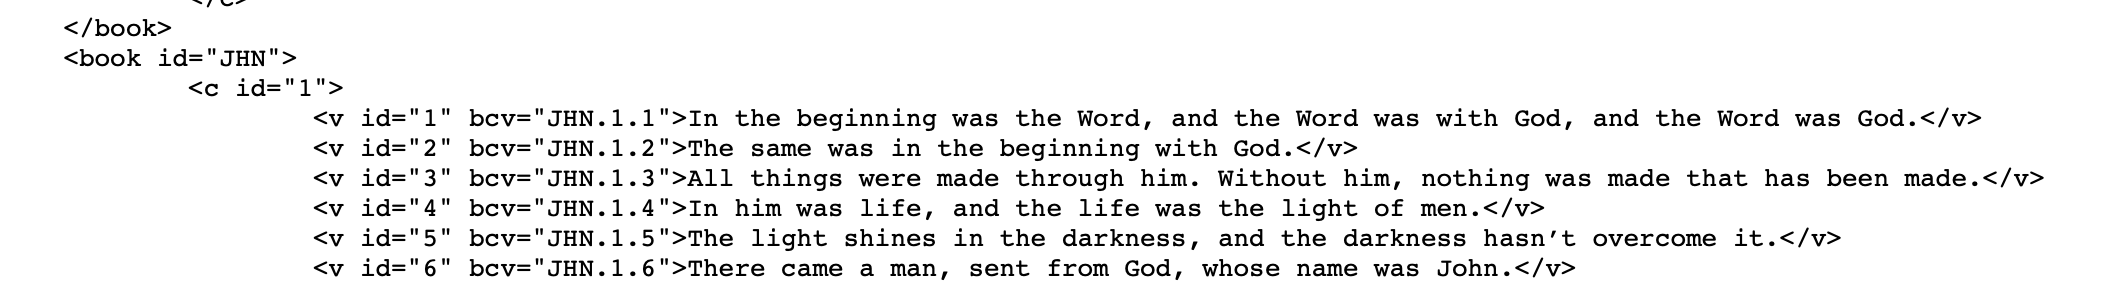
\includegraphics[width=\linewidth]{img/john_xml.png}
\end{frame}

\begin{frame}{Les sciences numériques et la critique textuelle}
    \textbf{Utilisation des sciences mathématiques/informatiques}:
    \begin{itemize}
        \item Transcriptions automatiques des manuscrits à l'aide des méthodes d'apprentissage profond;
        \item Décision automatique des leçons à l'aide de l'algorithme CBGM.
    \end{itemize}

    \begin{figure}
        \centering
        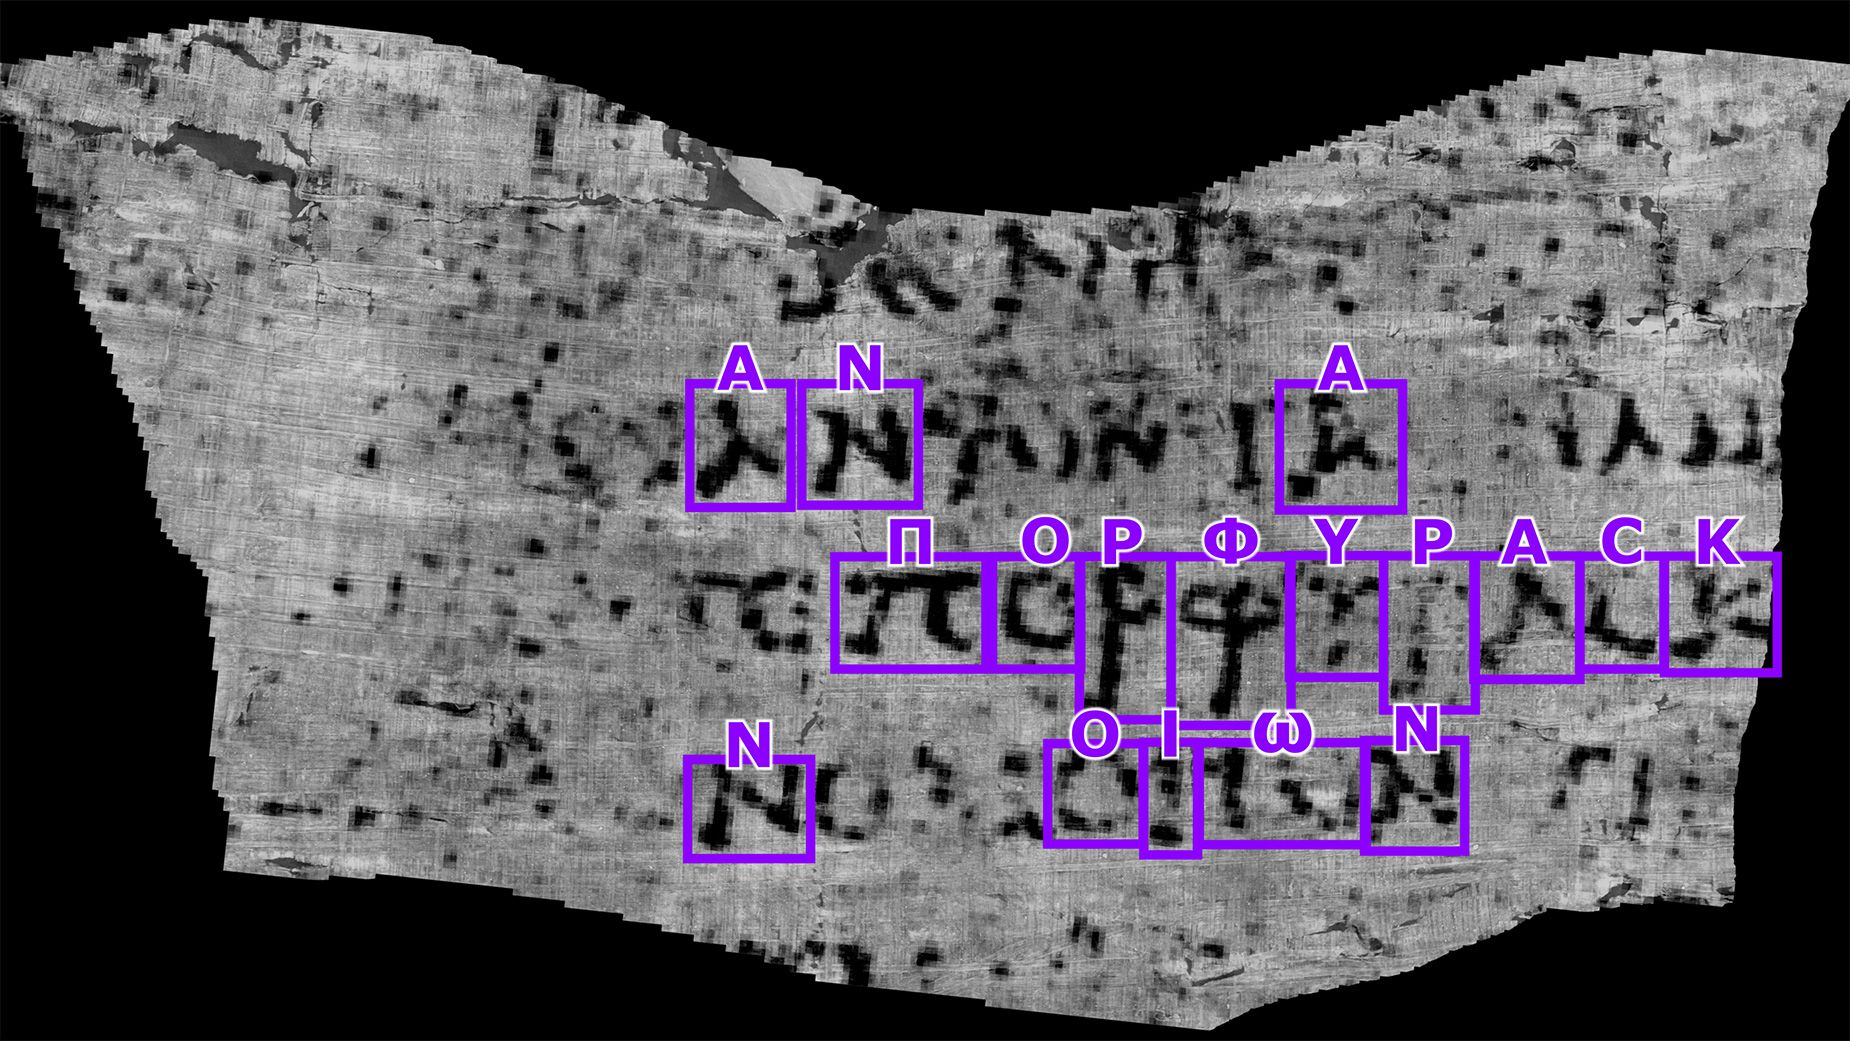
\includegraphics[width=0.5\linewidth]{img/vision_papyrus.JPG}
    \end{figure}
\end{frame}

\begin{frame}{}
Questions ?
\end{frame}

\end{document}